% Original PDF pages 378, 381, 385, 388, 391, 394, 397, and 406.
% The original data curves and patient icons are retained where used;
% Chinese labels are overlaid by TeX without changing the source assets.
\definecolor{chTwelveBand}{RGB}{185,204,234}
\definecolor{chTwelveCream}{RGB}{247,246,218}
\providecommand{\chTwelveFactorial}{\begin{tikzpicture}[font=\footnotesize,>=Stealth]
\draw[dashed,dcrred](0,0)ellipse(2.4 and 2.5);\node[text=dcrred]at(0,2.8){可接触人群};\node at(0,1.9){符合选择标准的参与者};
\node[draw=dcrred,text width=34mm,minimum height=29mm,align=center,text=dcrpurple](b)at(0,0){测量基线变量\\保存标本（可选）};
\node[circle,draw,minimum size=10mm](r)at(3.4,0){R};\draw[->](b)--(r);
\node[draw=dcrgold,text=dcrgold,align=center,text width=18mm,minimum height=83mm]at(10.95,0){也可于\\随访结束时\\测量结局};
\foreach \yy/\txt in {3.6/药物A＋药物B,1.2/药物A＋安慰剂B,-1.2/安慰剂A＋药物B,-3.6/安慰剂A＋安慰剂B}{
\node[draw=dcrteal,align=center,text width=43mm](a)at(7.4,\yy){\textcolor{dcrblue}{给予\txt}\\\textcolor{dcrgold}{结局发生时测量}};
\draw[->,dcrteal](r)to[bend left=12](a);\draw[->,dcrteal](a.east)--(9.95,\yy);
\foreach \xx in {7,8.2}{\draw[->,dcrteal](\xx,\yy-.5)to[bend left=25](\xx+.5,\yy-1);}\node[text=dcrteal]at(7.4,\yy-1.1){失访};}
\end{tikzpicture}}
\providecommand{\chTwelveNoninferiority}{\begin{tikzpicture}[x=.023cm,y=-.023cm]
\node[anchor=north west,inner sep=0]at(0,0){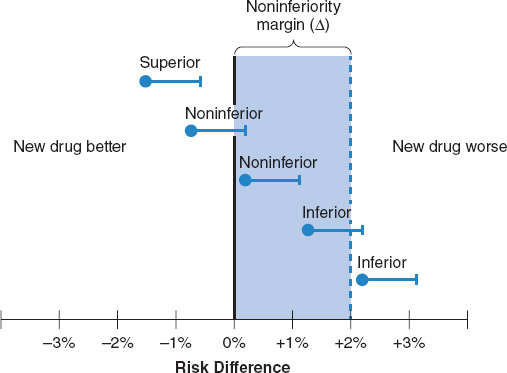
\includegraphics[width=11.661cm]{assets/ch12_figure02_original.png}};
\fill[white](230,0)rectangle(356,37);\node[font=\small,align=center]at(293,15){非劣效界值\\（$\Delta$）};
\fill[white](132,51)rectangle(205,72);\node[font=\small]at(169,62){优效};
\fill[white](176,102)rectangle(234,126);\fill[chTwelveBand](235,102)rectangle(282,126);\node[font=\small]at(220,115){非劣效};
\fill[chTwelveBand](236,152)rectangle(335,177);\node[font=\small]at(275,165){非劣效};
\fill[chTwelveBand](290,201)rectangle(350,224);\fill[white](351,201)rectangle(368,224);\node[font=\small]at(325,215){劣效};
\fill[white](352,251)rectangle(430,274);\node[font=\small]at(388,265){劣效};
\fill[white](10,135)rectangle(156,157);\node[font=\small]at(83,147){新药更好};
\fill[white](380,130)rectangle(512,165);\node[font=\small]at(448,147){新药更差};
\fill[white](150,353)rectangle(330,380);\node[font=\small]at(238,366){风险差};
\draw[dashed,dcrblue,line width=.8pt](350,55)--(350,319);
\end{tikzpicture}}
\providecommand{\chTwelveCrossover}{\begin{tikzpicture}[font=\footnotesize,>=Stealth]
\draw[dashed,dcrred](0,0)ellipse(1.75 and 2.4);\node[text=dcrred]at(0,2.65){可接触人群};\node[align=center]at(0,1.75){符合选择标准的样本};
\node[draw=dcrred,text width=23mm,align=center](b)at(0,0){测量基线预测变量\\及适当情况下的\\结局基线值};
\node[circle,draw](r)at(2.3,0){R};\draw[->](b)--(r);
\foreach \yy/\txt/\nm in {1.6/设盲干预/ctop,-1.6/设盲对照/cbottom}{\node[draw=dcrteal,text width=19mm,align=center](\nm)at(4.1,\yy){实施\txt};\draw[->,dcrteal](r)--(\nm);}
\node[draw=dcrgold,minimum height=43mm,align=center](m)at(5.8,0){测\\量\\结\\局};
\node[draw,minimum height=43mm,align=center](w)at(6.7,0){洗\\脱\\期};
\draw[->,dcrteal](ctop.east)--(5.55,1.6);\draw[->,dcrteal](cbottom.east)--(5.55,-1.6);
\node[draw=dcrteal,text width=19mm,align=center](a)at(8.6,1.6){实施设盲干预};\node[draw=dcrteal,text width=19mm,align=center](c)at(8.6,-1.6){实施设盲对照};
\draw[->,dashed,dcrteal](5.2,1.6)--(7.5,-1.6);\draw[->,dashed,dcrteal](5.2,-1.6)--(7.5,1.6);
\node[draw=dcrgold,minimum height=43mm,align=center](e)at(10.3,0){测\\量\\结\\局};\draw[->](a)--(e);\draw[->](c)--(e);
\foreach \x in {4,8.5}{\draw[->,dcrteal](\x+.5,1.2)to[bend left=25](\x+.8,.6);\node[text=dcrteal]at(\x,.45){失访};\draw[->,dcrteal](\x+.5,-2)to[bend left=25](\x+.8,-2.6);\node[text=dcrteal]at(\x,-2.7){失访};}
\end{tikzpicture}}
\providecommand{\chTwelveCluster}{\begin{tikzpicture}[x=.018cm,y=-.018cm]
\node[anchor=north west,inner sep=0]at(0,0){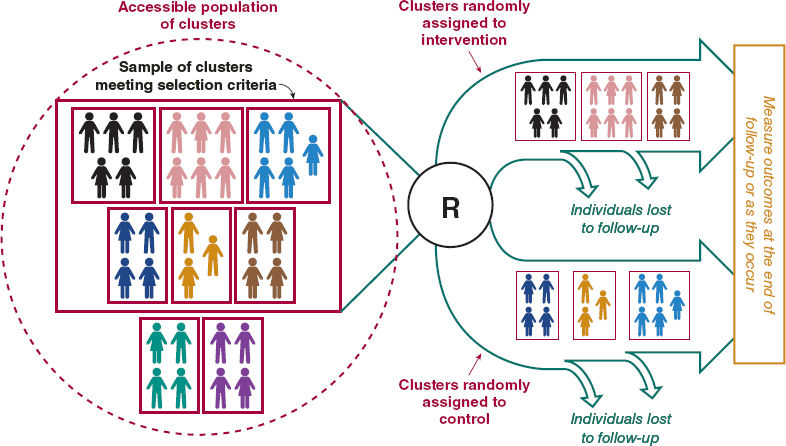
\includegraphics[width=14.148cm]{assets/ch12_figure04_original.png}};
\fill[white](108,0)rectangle(309,32);\node[font=\small]at(208,15){可接触人群中的群体};
\fill[white](91,55)rectangle(305,93);\node[font=\small,align=center]at(198,75){符合选择标准的群体样本};
\fill[white](395,0)rectangle(535,47);\node[font=\scriptsize,align=center,text=dcrred]at(465,22){随机分到\\干预的群体};
\fill[white](397,378)rectangle(535,427);\node[font=\scriptsize,align=center,text=dcrred]at(465,401){随机分到\\对照的群体};
\fill[white](550,198)rectangle(720,240);\node[font=\scriptsize,text=dcrteal]at(635,216){个体失访};
\fill[white](550,412)rectangle(720,451);\node[font=\scriptsize,text=dcrteal]at(635,430){个体失访};
\fill[white](737,48)rectangle(783,361);\node[font=\scriptsize,rotate=90,text=dcrgold]at(760,205){结局发生时或随访结束时测量结局};
\end{tikzpicture}}
\providecommand{\chTwelveStepped}{\begin{tikzpicture}[font=\footnotesize,x=.58cm,y=.42cm]
\foreach \row/\lab in {0/9,1/3,2/12,3/7,4/8,5/5,6/11,7/2,8/10,9/1,10/4,11/5}{
\node[anchor=east]at(0,-\row-.5){群\lab};
\pgfmathtruncatemacro{\start}{2*floor(\row/2)+3}
\foreach \col in {1,...,14}{\ifnum\col<\start\fill[white](\col-1,-\row)rectangle(\col,-\row-1);\else\fill[chTwelveBand](\col-1,-\row)rectangle(\col,-\row-1);\fi\draw[dcrblue,thin](\col-1,-\row)rectangle(\col,-\row-1);}}
\foreach \col in {1,...,14}{\node at(\col-.5,-12.6){\col};}
\foreach \col in {1,3,5,7,9,11,13}{\draw[dcrred](\col,-12)--(\col,0);}
\node at(7,-13.4){月};\draw[->,dcrblue](0,-14)--(0,-12.1);\node[anchor=east]at(0,-14.2){试验开始};\draw[->,dcrblue](14,-14)--(14,-12.1);\node[anchor=west]at(14,-14.2){试验结束};
\end{tikzpicture}}
\providecommand{\chTwelveBefore}{\begin{tikzpicture}[font=\small,>=Stealth]
\draw[dashed,dcrred](0,0)ellipse(2.3 and 2.4);\node[text=dcrred]at(0,2.7){可接触人群};\node[align=center]at(0,1.8){符合选择标准的参与者};
\node[draw=dcrred,text width=33mm,minimum height=27mm,align=center](b)at(0,0){\textcolor{dcrpurple}{测量基线预测变量}\\\textcolor{dcrgold}{测量结局基线值}};
\draw[->,thick,dcrteal](b)--node[above]{实施干预}(8,0);\node[draw=dcrgold,text=dcrgold,align=center]at(8.8,0){测量\\结局变量};
\foreach \x in {3.5,6}{\draw[->,dcrteal](\x,0)to[bend left=30](\x+.5,-1.6);}\node[text=dcrteal]at(5,-2){失访};
\draw[->,thick,dcrteal](1.8,-3)--(8.8,-3);\node[fill=white,text=dcrteal]at(5,-3){随访时间};\node[align=center]at(0,-3.2){研究起始\\（之前）};\node[align=center]at(9,-3.7){研究结束\\（之后）};
\end{tikzpicture}}
\providecommand{\chTwelveTimeSeries}{\begin{tikzpicture}[x=.026cm,y=-.026cm]
\node[anchor=north west,inner sep=0]at(0,0){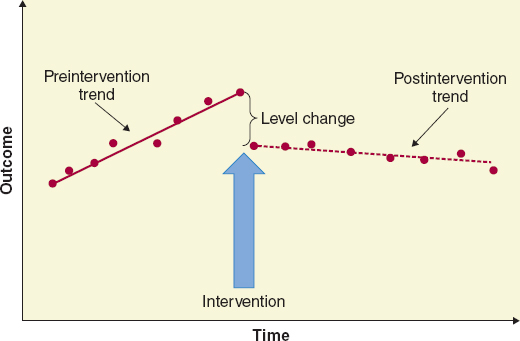
\includegraphics[width=13.52cm]{assets/ch12_figure07_original.png}};
\fill[chTwelveCream](40,64)rectangle(155,108);\node[font=\small,align=center]at(100,85){干预前趋势};
\fill[chTwelveCream](260,105)rectangle(380,135);\node[font=\small]at(320,120){水平变化};
\fill[chTwelveCream](390,65)rectangle(511,108);\node[font=\small]at(449,85){干预后趋势};
\fill[chTwelveCream](194,289)rectangle(293,316);\node[font=\small]at(244,302){干预};
\fill[white](0,122)rectangle(17,198);\node[font=\small,rotate=90]at(8,162){结局};
\fill[white](240,322)rectangle(315,345);\node[font=\small]at(277,333){时间};
\end{tikzpicture}}
\providecommand{\chTwelvePriors}{\begin{tikzpicture}[x=.0198cm,y=-.0198cm]
\node[anchor=north west,inner sep=0]at(0,0){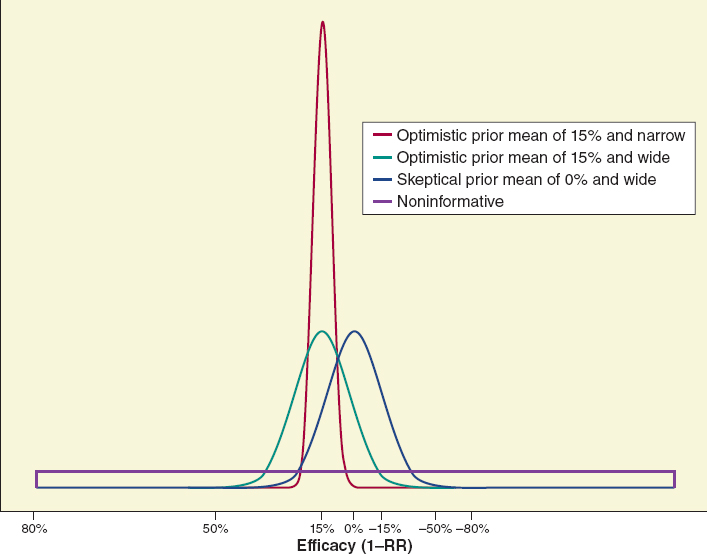
\includegraphics[width=13.9986cm]{assets/ch12_figurea01_original.png}};
\fill[white](396,124)rectangle(693,210);
\node[anchor=west,font=\scriptsize]at(398,136){乐观先验：均值15\%，分布窄};
\node[anchor=west,font=\scriptsize]at(398,158){乐观先验：均值15\%，分布宽};
\node[anchor=west,font=\scriptsize]at(398,180){怀疑先验：均值0\%，分布宽};
\node[anchor=west,font=\scriptsize]at(398,202){无信息先验};
\fill[white](292,536)rectangle(415,554);\node[font=\small]at(354,546){疗效（$1-\mathrm{RR}$）};
\end{tikzpicture}}
